\documentclass[9pt,lineno,doublespacing]{elife}
\usepackage{nameref}
\usepackage{setspace}
\usepackage{booktabs}
\usepackage{colortbl}
\usepackage{mathtools}
\usepackage{siunitx}
\usepackage{tabularx}
\usepackage{todonotes}
\usepackage{tikz}
\usepackage{chemfig}

% glossaries. Disable the link in main document.
\usepackage[acronym]{glossaries}
\loadglsentries{glossaries}
\usepackage{siunitx}
\DeclareSIUnit\Molar{M}
\glsdisablehyper

\title{Subunit exchange enhances information retention by CaMKII in dendritic spines}

\author[]{Dilawar Singh}
\author[]{Upinder Singh Bhalla}

\affil[]{National Centre for Biological Sciences Bangalore, Tata Institute of Fundamental Research}
\corr{bhalla@ncbs.res.in}{USB}

\presentadd[]{National Centre of Biological Sciences Bangalore, Tata Institute of Fundamental Research, India
}

% macros for superscript and subscript.
\newcommand\SUB[2]{#1\textsubscript{#2}}
\newcommand\SUP[2]{#1\textsuperscript{#2}}

% Document begins here.
\begin{document}
\maketitle

% ABSTRACT
\begin{abstract}\label{abstract} 
Molecular bistables are strong candidates for long-term information storage, for
example, in synaptic plasticity. Calcium/calmodulin dependent protein Kinase II
(CaMKII) is a highly expressed synaptic protein which has been proposed to form
a molecular bistable switch capable of maintaining its state for years despite
protein turnover and stochastic noise. It has recently been shown that CaMKII
holoenzymes exchange subunits among themselves. Here we used computational
methods to analyze the effect of subunit exchange on the CaMKII pathway in the
presence of diffusion in two different micro-environments, the Post Synaptic
Density (PSD) and spine cytosol. We show that CaMKII exhibits multiple 
timescales of activity due to subunit exchange. Further,
subunit exchange enhances information retention by CaMKII both by
improving the stability of its switching in the PSD, and by slowing the decay of
its activity in the spine cytosol. The existence of diverse timescales in the
synapse has important theoretical implications for memory storage in networks.
\end{abstract}

\section{Introduction}\label{introduction}

Memories are believed to be stored in synapses, encoded as changes in synaptic
strength \citep{hebb_organization_2005,takeuchi_synaptic_2014,choi_interregional_2018}.
\gls{ltp}, an activity dependent change in synaptic strength, is considered to
be the primary post-synaptic memory mechanism
\citep{bliss_expression_2013,mayford_synapses_2012}. Various behavioural
experiments strongly suggest a critical role for \gls{camkii} in induction of
\gls{ltp} \citep{lucchesi_novel_2011,giese_autophosphorylation_1998}. In
the CA1 region of Hippocampus, blocking \gls{camkii} activity blocks the
induction of \gls{ltp} \citep{chang_camkii_2017}. After LTP induction, several
other pathways including protein synthesis \citep{aslam_translational_2009},
clustering of receptors \citep{shouval_clusters_2005}, receptor translocation
\citep{hayer_molecular_2005} and PKM-$\zeta$ activation
\citep{sacktor_memory_2012}, have been suggested as mechanisms for long-term
maintenance of synaptic state. Recent evidence from behavioural assays suggests
that \gls{camkii} may also be involved in long-term maintenance of memory
\citep{rossetti_memory_2017} (but see \citep{chang_camkii_2017}).

Any putative molecular mechanism involved in long-term maintenance of memory
must be able to maintain its state despite the potent resetting mechanisms of
chemical noise and protein turnover. In the small volume of the synapse ($\sim$
0.02 \si{\micro\meter^3} \citep{bartol_nanoconnectomic_2015}), the number of
molecules involved in biochemical processes range from single digits to a few
hundred, thereby increasing the effect of chemical noise. John Lisman proposed that
a kinase and its phosphatase could form a bistable molecular switch able to
maintain its state for a very long time despite turnover
\citep{lisman_mechanism_1985}. It has been shown by various mathematical models
that \gls{camkii} and its phosphatase \gls{pp1} may form a bistable switch
\citep{zhabotinsky_bistability_2000} which can retain its state for years
despite stochastic chemical noise and protein turnover
\citep{miller_stability_2005}. Although there is experimental evidence that
CaMKII/PP1 is bistable in \emph{in vitro} settings
\citep{bradshaw_ultrasensitive_2003,urakubo_vitro_2014}, experimental evidence
for \emph{in vivo} bistability is lacking. In spine cytosol, \gls{camkii} has
been shown not to act like a bistable switch but rather a leaky integrator of
calcium activity \citep{chang_camkii_2017}. However, \gls{camkii} may be
bistable in special micro-environments such as the ``core'' \gls{psd} where it
attaches to NMDA receptor \citep{dosemeci_postsynaptic_2016,
petersen_distribution_2003}.

From a computational perspective, the CaMKII/PP1 bistable system is an attractive
candidate for memory storage \citep{koch_biophysics_2004}. Bistability provides
a plausible solution to the problem of state maintenance. Previous modeling work
has shown that the CaMKII/PP1 system may form a very stable switch despite protein 
turnover and stochastic noise in the small volume of the synapse. The stability
increases exponentially with the number of holoenzymes
\citep{miller_stability_2005}. It is important to note that this model exhibits
bistable behaviour only in a narrow range of \gls{pp1} concentrations in the
\gls{psd}. This strict restriction may be met because phosphorylated
\gls{camkii} is protected from phosphatases in \gls{psd} except \gls{pp1}
\citep{strack_differential_1997} which is tightly regulated in the \gls{psd}
\citep{bollen_extended_2010}. 

\gls{camkii} has another remarkable property which was hypothesized by Lisman
\citep{lisman_cam_1994} but discovered only recently, namely, subunit exchange.
In this process, two \gls{camkii} holoenzymes can exchange active subunits
leading to spread of \gls{camkii} activation \citep{stratton_activation-triggered_2014}.

In this paper, we adapt the \gls{mz} \citep{miller_stability_2005} to include
subunit exchange and diffusion, and quantify the effects of subunit exchange on
the properties of the \gls{camkii}-\gls{pp1} PP1 system in two adjacent neuronal
micro-environments: \gls{psd} and spine cytosol. 

In the \gls{psd}, \gls{pp1} is tightly regulated and \gls{camkii} is protected
from other phosphatases. But in the spine cytosol, \gls{camkii} is accessible to
other phosphatases along with \gls{pp1}. We examined how state switching
lifetimes in the \gls{psd} are affected by subunit exchange in different
contexts of \gls{pp1} levels, turnover, and clustering of \gls{camkii}. In the
spine cytosol we show how the integration of calcium stimuli generates two
time-courses of \gls{camkii} activity as a result of subunit exchange
\citep{chang_camkii_2017}.

% RESULTS
\section{Results}\label{sec:results} 
\subsection{Model validation}\label{subsec:model-validation}
The basic computational units in our model are individual \gls{camkii} subunits,
and \gls{camkii} ring consisting of 6 or 7 \gls{camkii} subunits. We treat the
\gls{camkii} ring as a proxy for the \gls{camkii} holoenzyme, which consists of
two such rings stacked over each other
\citep{woodgett_calmodulin-dependent_1983,hoelz_crystal_2003,chao_mechanism_2011}. In
our model, \gls{camkii} exists in 15 possible states compared to 2 in the
\gls{mz} model (see \nameref{sec:materials_and_methods}). This leads to many
more reactions than the \gls{mz} model. We also replaced Michaelis-Menten
approximation in the \gls{mz} model by equivalent mass-action kinetics (e.g.,
\EQ{dephosphorylation}).  Since analytical comparison of the two models was not
possible, we first compared numerical results from our model without diffusion
and without subunit exchange with the \gls{mz} model (\FIG{validation}).

Our model exhibited all the key properties of the \gls{mz} model: 1. In
\gls{psd}, under basal \gls{ca} stimulus conditions, CaMKII/PP1 formed a
bistable switch (\FIG{validation}C, D), 2. The stability of the switch increased
exponentially with system size (\FIG{validation}E), 3. Increased number of
\gls{pp1} molecules (\SUB{N}{PP1}) shut off the switch (\FIG{tolerance_pp1}),
and, 4. Bistability was robust to slow turnover of \gls{camkii}
(\FIG{turnover}).

Thus, our baseline model exhibited all the key properties that had
previously been predicted for the bistable \gls{camkii} switch. However, 
subunit exchange and diffusion introduced several interesting additional
properties, which we examine below.

\begin{figure}[t]%[hbt] 
    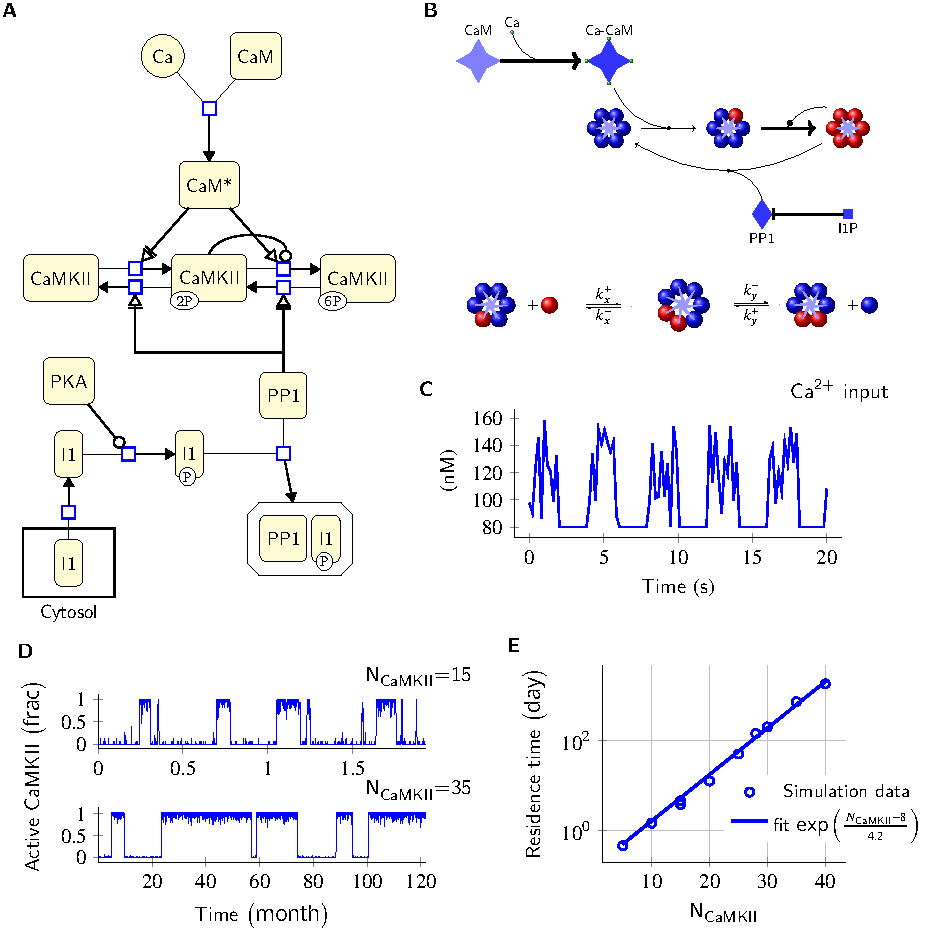
\includegraphics[width=0.95\linewidth]{./PaperFigures/elifeFigure1/figure_validation_178mm.pdf}
    \caption{Model description and validation. \textbf{(A)} CaMKII/PP1 pathway
        described in \gls{sbgn} - Process Description (PD) Language
        \citep{novere_systems_2009}. \textbf{(B)} \textbf{(above)} Major
        chemical reactions in the CaMKII/PP1 pathway. \textbf{(below)} Subunit
        exchange between two \gls{camkii} holoenzymes. Blue and red balls
        represent phosphorylated and un-phosphorylated subunits respectively.
        \textbf{(C)} Basal \gls{ca} profile in spine and \gls{psd}. Basal
        \gls{ca} level is \SI{80}{\nano M} with fluctuations every
        \SI{2}{\second}, lasting for \SI{2}{\second}. These fluctuations
        (represented by symbol $\epsilon$) are sampled from a uniform distribution with median of
        \SI{120}{\nano M} and range of \SI{40}{\nano M} (see
        \nameref{sec:materials_and_methods}). \textbf{(D)} Without diffusion and subunit exchange,
        CaMKII in our model is bistable. Two trajectories of \gls{camkii}
        activity (fraction of total \gls{camkii} holoenzymes with at least 2
        subunits phosphorylated) are shown for different system sizes
        \SUB{N}{CaMKII}=15 (\textbf{top}) and \SUB{N}{CaMKII}=35
        (\textbf{bottom}). \textbf{(E)} Switch stability measured as average
        residence time of its stable states increases exponentially with system
        size \SUB{N}{CaMKII}. Turnover rate \SUB{v}{t}=\SI{30}{\per \hour}.
        Panels \textbf{C, D}, and \textbf{E} show key properties of our model
        that are very similar to those of the \gls{mz} model.
    }\label{fig:validation} 
    \figdata{Source and data are available at
    \url{http://github.com/dilawar/SinghAndBhalla_CaMKII_SubunitExchange_2018/tree/master/PaperFigures/elifeFigure1}}
\end{figure}


\subsection{Subunit exchange increases the tolerance of the CaMKII switch to PP1
and to turnover}\label{subsec:result_tolerance}

\begin{figure}[ht]
    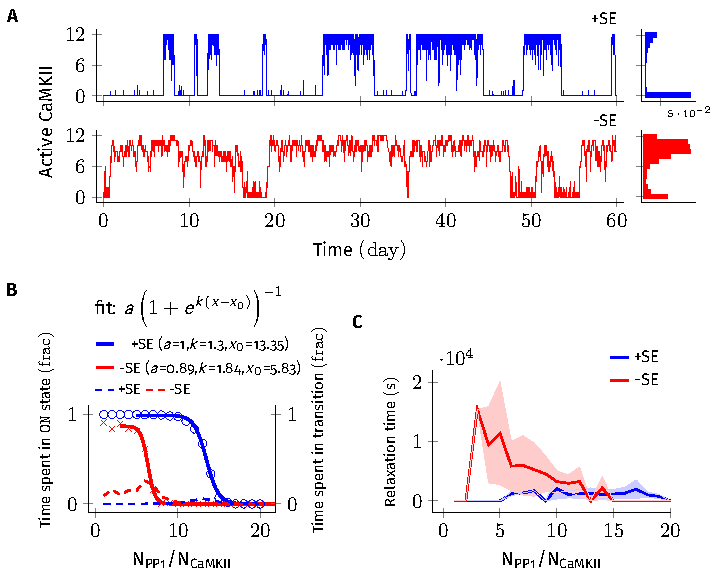
\includegraphics[width=140mm]{PaperFigures/elifeFigure2/figure_effect_of_tolerace_140mm.pdf}
    \caption{Subunit exchange improves the switch's tolerance of \gls{pp1} by
        acting as a compensatory mechanism for the dephosphorylation by \gls{pp1} 
        \textbf{(A)} Two representative trajectories (\SUB{N}{CaMKII}=12) are
        shown with subunit exchange (+SE, blue) and without
        subunit exchange (-SE, red) respectively. \textbf{(B)} Blue and red
        solid-lines represent average activity of switch with and without 
        subunit exchange respectively. The lines are fitted with the 
        function \({a}/\left({1+e^{k(x-x_0)}}\right)\).
        Dotted red and blue lines show the fraction of time that the switch
        spends in intermediate states (\SUB{x}{a}\SUB{y}{n-a}, 1<a<n-1) with
        and without subunit exchange respectively. Due to subunit exchange,
        the switch tolerated a larger amount of \gls{pp1} 
        (\SUB{x}{0} value 11.2 vs 17.77 i.e., a change of 6.57$\times$\SUB{N}{CaMKII}).
        Note that the range of \gls{pp1} for which switch remains bistable is roughly the 
        same (k, 0.6 v/s 0.58). The fraction of time in intermediate states (dotted lines)
	is much smaller when subunit exchange is enabled (blue dotted line),
        i.e., the switching time is shorter. \textbf{(C)} Due to subunit exchange, relaxation 
        time becomes constant and independent of \SUB{N}{PP1} (blue vs red). 
        Shaded area represents standard deviation.
    }\label{fig:tolerance_pp1}
    \figdata{Source and data are available at
    \url{http://github.com/dilawar/SinghAndBhalla_CaMKII_SubunitExchange_2018/tree/master/PaperFigures/elifeFigure2}}
\end{figure}

We first analyzed switch sensitivity to \gls{pp1}. In our model as well in the
\gls{mz} model, the number of PP1 molecules (\SUB{N}{PP1}) has an upper limit
for the switch to exhibit bistability. This constraint arises because \gls{pp1}
must saturate in the \texttt{ON} state of the switch, i.e., the maximal
enzymatic turnover of \gls{pp1} must be smaller than the rate of activation of
\gls{camkii} subunits. However, unlike the \gls{mz} model where the addition of
one extra \gls{pp1} molecule changed the residence time of the \texttt{ON} state by
roughly 90\% (Figure~2C in \citep{miller_stability_2005}), we did not find the
residence time of the \texttt{ON} state to be this sensitive to \gls{pp1}. In our
model, on average it required 0.5$\times$\SUB{N}{CaMKII} extra \gls{pp1}
molecules to cause a similar 90\% change in the residence time of the \texttt{ON}
state.  This number is roughly equal to the maximum number of \gls{camkii}
subunits (released from \gls{camkii} holoenzymes during subunit exchange
\EQ{losegainx}) that can exist at any given time in our model. We conjecture
that this reduced sensitivity to \gls{pp1} is due to the fact that \gls{pp1}
participates in many more reactions in our model. 

We found that a system consisting of \SUB{N}{CaMKII} holoenzymes remained
bistable for \SUB{N}{PP1}=8$\times$ to 15$\times$\SUB{N}{CaMKII} without subunit
exchange, and for \SUB{N}{PP1}=12$\times$ to 21$\times$\SUB{N}{CaMKII} with
subunit exchange. Thus, subunit exchange shifted the bistable range to higher
values of \gls{pp1}. Nevertheless, the gap between the upper and lower limit remained
the same in both cases (blue and red sigmoidal fit in \FIG{tolerance_pp1}B).

In the presence of subunit exchange, the \texttt{ON} state of switch has a
tighter distribution (blue v/s red histogram, \FIG{tolerance_pp1}A), i.e., there
are fewer holoenzymes that are completely de-phosphorylated by \gls{pp1}. We
interpret this as follows: In the presence of subunit exchange, any subunit in a
holoenzyme de-phosphorylated by the \gls{pp1} is likely to be rapidly
re-phosphorylated. This is because, when the switch is in \texttt{ON} state,
most subunits present in the \gls{psd} are in the phosphorylated state. Hence,
in addition to auto-phosphorylation, the exchange reactions (\EQ{losegainx})
turn unphosphorylated holoenzymes to phosphorylated holoenzymes with a
significant rate (data not shown). Taken together, subunit exchange acts as a
compensatory mechanism for dephosphorylation by \gls{pp1} in the \texttt{ON}
state of the switch.

Subunit exchange also had a strong effect on time spent by the switch in
transition from one stable state to another (relaxation time). When subunit
exchange was enabled, the relaxation time was reduced (red v/s blue dotted line
in \FIG{tolerance_pp1}B) and also became independent of \SUB{N}{PP1}. As
mentioned previously, due to subunit exchange, the \texttt{ON} state has a
tighter distribution (blue v/s red histogram in \FIG{tolerance_pp1}A). This
means that there were fewer ineffective transitions from the \texttt{ON} to the
\texttt{OFF} state. As expected, the standard deviation of the relaxation time
was also greatly reduced in the presence of subunit exchange (red and blue
curve, \FIG{tolerance_pp1}C). Thus subunit exchange makes the switch's
\texttt{ON} state less noisy and more robust to dephosphorylation by \gls{pp1}.

Parallel results were obtained for the effect of subunit exchange on
\gls{camkii} switch robustness in the context of protein turnover. Turnover
replaces any active \gls{camkii} holoenzyme by an inactive holoenzyme with a
constant rate (\EQ{turnover}), thus decreasing the stability of the \texttt{ON}
state. Without subunit exchange, switch stability as measured by residence time
of the \texttt{ON} state decreased exponentially with increasing turnover rate.
With subunit exchange, however, residence time of the \texttt{ON} state remained
roughly constant upto a $\sim$10 fold increase in turnover (\FIG{turnover}B),
after which subunit exchange could not phosphorylate all inactive holoenzymes
produced by turnover. At this point the switch started to show a similar steep
decay of stability as was seen without subunit exchange. As expected, turnover
increased the number of switching events in the regime of bistability in both
cases.

\begin{figure}[th!]
    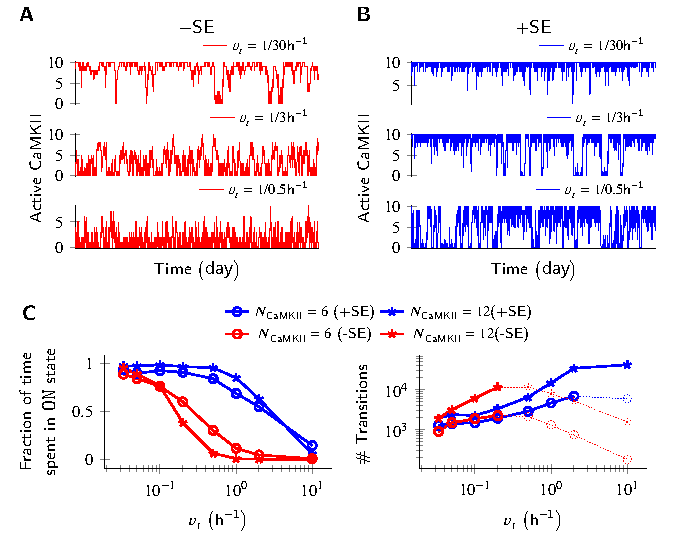
\includegraphics[width=114mm]{./PaperFigures/elifeFigure3/figure_turnover_tolerance_114.pdf}
    \caption{Subunit exchange improves switch tolerance of higher rates of
        protein turnover.
        \textbf{(A,B)} Three sample trajectories are shown for a switch of 
        size \SUB{N}{CaMKII}=10 without subunit exchange
        (-SE,red) and with it (+SE,blue). We consider three different 
        turnover rates of 1 per \SI{30}{\hour}, 1 per \SI{3}{\hour}, 
        and 1 per 0.5 \si{\hour}. As turnover is increased, the state stability 
        of the \texttt{ON} state of the switch decreases.
        \textbf{(C, left)} Normalized residence time of the \texttt{ON} state v/s turnover
        rate for two switches of size 6 and 12. Without subunit exchange, switch
        stability decreases steeply with turnover rate (red), however when
        subunit exchange is enabled, switch stability is not affected by
        turnover rates as high as \SI{1}{\per \hour} (blue). \textbf{(C,right)} In
        the bistable regime (solid lines), the number of switching events
        increases monotonically with turnover rate.
    }\label{fig:turnover}
    \figdata{Source and data are available at
    \url{http://github.com/dilawar/SinghAndBhalla_CaMKII_SubunitExchange_2018/tree/master/PaperFigures/elifeFigure3}}
\end{figure}

Thus, subunit exchange increases the range of \SUB{N}{PP1} and turnover rate
over which the switch remains bistable. It also reduces fluctuations in the
switch's \texttt{ON} state.

\subsection{Subunit exchange facilitates the spread of CaMKII activity}
\label{res:spread_activity}

As suggested in \citep{stratton_activation-triggered_2014}, we found that
subunit exchange facilitated the spread of \gls{camkii} activation
(\FIG{subunit_facilitates_spread}). When subunits were allowed to diffuse, an
active subunit could be picked by a neighbouring inactive \gls{camkii}
holoenzyme, making it partially phosphorylated. This process overcomes the first
slow step of \gls{camkii} phosphorylation (\EQ{phospho}), especially when
subunit exchange makes many phosphorylated subunits available, thereby
facilitating the spread of activation.

We simulated \SUB{N}{CaMKII}=18 inactive holoenzymes in a cylinderical arena
with a volume of \SI{0.0275}{\cubic\micro\meter} and a length of
\SI{540}{\nano\meter} representing the \gls{psd}. The cylinder was divided into
18 voxels (1 holoenzyme in each voxel). Each voxel was separated by
\SI{30}{\nano\meter}, which is the average nearest-neighbour distance for
\gls{camkii} holoenzymes \citep{feng_quantitative_2011}. Each voxel was
considered to be a \emph{well-mixed} environment i.e., diffusion was
instantaneous within the voxel. Between voxels, diffusion was implemented as
cross-voxel ``jump'' reactions (See \nameref{sec:materials_and_methods}). We did
not try 2D/3D diffusion because of its simulation complexity and because it
would be expected to be qualitatively similar \citep{fange_stochastic_2010}.

We fixed the diffusion coefficient of \gls{pp1} (\SUB{D}{PP1}) to quantify the
effect of varying the diffusion coefficient of subunits (\SUB{D}{sub}) and basal
calcium levels. We used \SUB{D}{PP1}=\SI{0.5}{\micro\meter\squared\per\second}
which is the observed value of the diffusion coefficient of Ras, a similar sized
protein \citep{harvey_spread_2008}. We ran simulations for 4 hours at basal
calcium concentration [\gls{ca}]=\SI{80}{\nano M}+$\epsilon$ (where $\epsilon$
is fluctuation in basal calcium levels \FIG{validation}C) and without subunit
exchange (i.e., \SUB{D}{sub}=0). We set \SUB{N}{PP1}=15$\times$\SUB{N}{CaMKII}
to make sure the system showed no significant \gls{camkii} activity
(\FIG{subunit_facilitates_spread}A, red curve). This served as the baseline to
quantify the effect of subunit exchange. When we enabled subunit exchange by
setting \SUB{D}{sub}=\SI{0.1}{\micro\meter\squared\per\second}, \gls{camkii}
activity rose to a maximum within \SI{4}{\hour} even when we used a low value
for \SUB{D}{sub}=\SI{0.001}{\micro\meter\squared\per\second}
(\FIG{subunit_facilitates_spread}C, black and brown curves).

As expected, at higher basal \gls{ca} level (\SI{120}{\nano M}), the system
showed higher \gls{camkii} activity for all values of \SUB{D}{sub}
(\FIG{subunit_facilitates_spread}D). Increasing \SUB{D}{sub} increased the
effect of subunit exchange, as measured by the decreased rise time of
\gls{camkii} activity from 10\% to 90\% (\FIG{subunit_facilitates_spread}D).
However the time of onset of \gls{camkii} activation as measured by rise time
from 0\% to 10\% was dependent only on basal \gls{ca} levels but not on
\SUB{D}{sub} (\FIG{subunit_facilitates_spread}E).

Thus, subunit exchange facilitates the spread of kinase activity following
\gls{camkii} activation but does not affect the onset of \gls{camkii}
activation.

\begin{figure}
    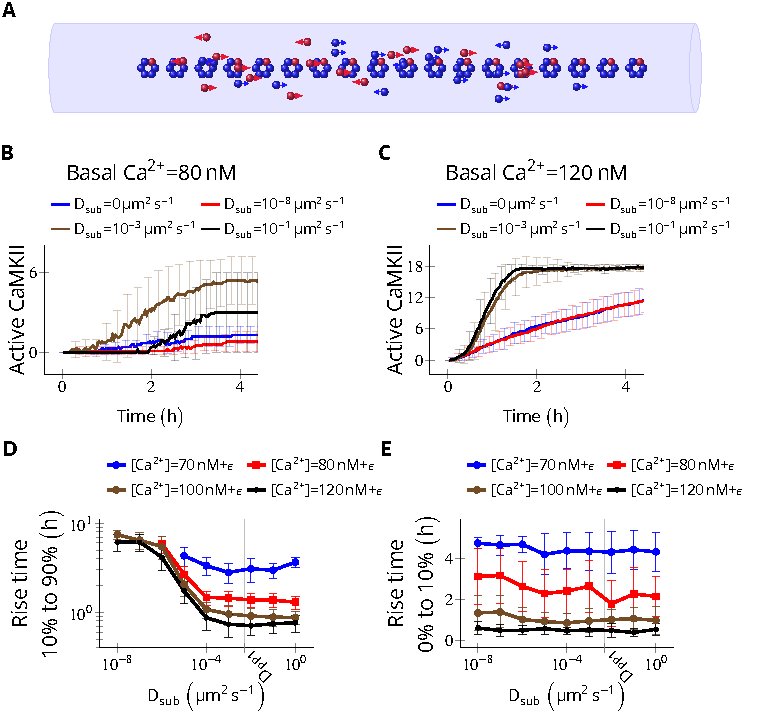
\includegraphics[width=0.95\linewidth]{./PaperFigures/elifeFigure4/figure_camkii_activation_130mm.pdf}
    \caption{Subunit exchange facilitates the spread of kinase activity
        \citep{stratton_activation-triggered_2014}. \textbf{(A)} 18 \gls{camkii}
        holoenzymes were simulated in a cylindrical arena of volume
        \SI{0.0275}{\cubic\micro\meter}, discretized into 18 voxels, each
        separated by \SI{30}{\nano\meter}. Red and blue balls represent
        unphosphorylated and phosphorylated subunits respectively.
        %
        \textbf{(B)} Activation profile of \gls{camkii} at mean basal calcium
        level of \SI{80}{\nano M}+$\epsilon$ ($\epsilon$ is fluctuation in basal
        \gls{ca} levels \FIG{validation}A) for various values of \SUB{D}{sub}
        with \SUB{N}{PP1}=15$\times$\SUB{N}{CaMKII}. For this value of
        \SUB{N}{PP1}, we see moderate or no mean activity of \gls{camkii} for
        various values of \SUB{D}{sub} for basal \gls{ca}=\SI{80}{\nano
        M}+$\epsilon$. This serves as the baseline for comparisons.
        %
        \textbf{(C)} At a slightly higher level of basal \gls{ca}
        (\SI{120}{\nano M}+$\epsilon$), subunit exchange has a stronger effect
        on \gls{camkii} activation. When subunits were modeled with zero or very
        small diffusion coefficients (\SUB{D}{sub}=0 and
        \SUB{D}{sub}=\SI{1e-8}{\micro\meter\squared\per\second}), the effect of
        subunit exchange was smaller than when subunits were tested with
        moderate to high diffusion coefficients (\SUB{D}{sub}=0.001 and 0.1
        \si{\micro\meter\squared\per\second}), 
        %
        \textbf{(D)} Quantification of effect of subunit exchange seen in
        \textbf{A} and \textbf{B} v/s \SUB{D}{sub} and basal \gls{ca} levels.
        The time taken by \gls{camkii} to rise from 10\% to 90\% of its maximum
        value (rise time) in hours v/s \SUB{D}{sub} for different mean basal
        calcium levels. The effect of subunit exchange is greater (as measured
        by shorter rise times) at higher calcium levels for all values of
        \SUB{D}{sub}. Rise time is also shorter for larger \SUB{D}{sub} for all
        values of [\gls{ca}].  Error bars represents standard deviation (n=40
        trajectories).
        %
        \textbf{(E)} The time to onset of \gls{camkii} activity is independent
        of \SUB{D}{sub} and depends only on [\gls{ca}]. The time to onset of
        activity is measured as the time taken by inactive \gls{camkii} to rise
        from zero to 10\% of its maximum value. Average time for the onset of
        activity decreased with increasing basal [\gls{ca}] levels but remained
        independent of \SUB{D}{sub} suggesting that subunit exchange does not
        play any significant role in the beginning of activation of \gls{camkii}
        by \gls{ca}. Error bar represents standard deviation (n=40 trajectories).
        \SUB{D}{PP1}=\SI{0.5}{\micro\meter\squared\per\second} for all simulations.
    }\label{fig:subunit_facilitates_spread} 
% first suppl
\figsupp[Sample trajectories of \gls{camkii} activation for basal \gls{ca}
concentration of \SI{100}{\nano M}+$\epsilon$.]{In all simulations, \SUB{D}{PP1}
    was set to \SI{0.5}{\micro\meter\squared\per\second} and \SUB{D}{sub} was
    varied.  Each plot contains 40 trajectories. Dark black trajectory in each
    plot shows the average trajectory.
}{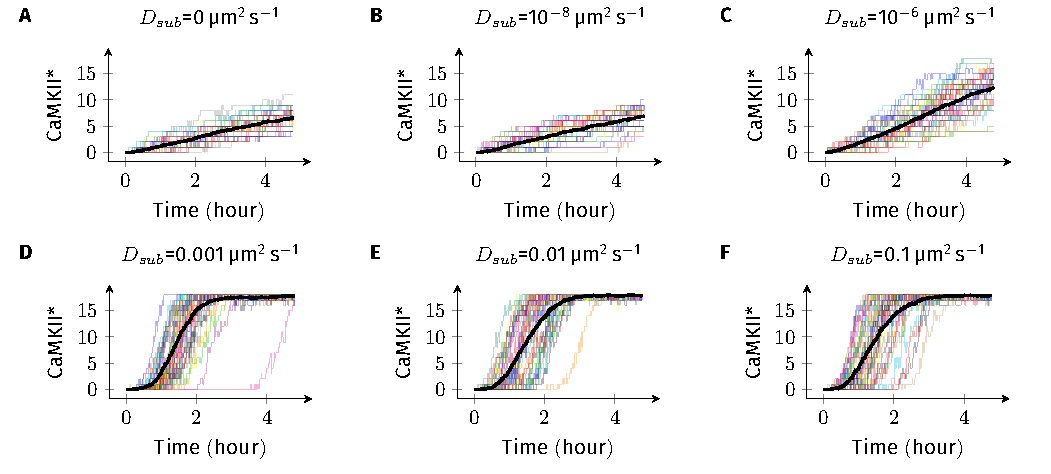
\includegraphics[width=\linewidth]{./PaperFigures/suppl/figure_camkii_activations_trajs.pdf}}
\label{figsupp:camkii_activation_se_trajs} \figdata{Source and data are
available at
\url{http://github.com/dilawar/SinghAndBhalla_CaMKII_SubunitExchange_2018/tree/master/PaperFigures/elifeFigure4}}
\end{figure}


%%%%%%%%%%%%%%%%%%%%%%%%%%%%%%%%%%%%%%%%%%%%%%%%%%%%%%%%%%%%%%%%%%%%%%%%%%%%%%%
% Spread of activity and synchronization

\subsection{Subunit exchange synchronizes switching activity of clustered CaMKII}
\label{subsec:se_sync_switches}

\begin{figure}%[t]%[bth] 
    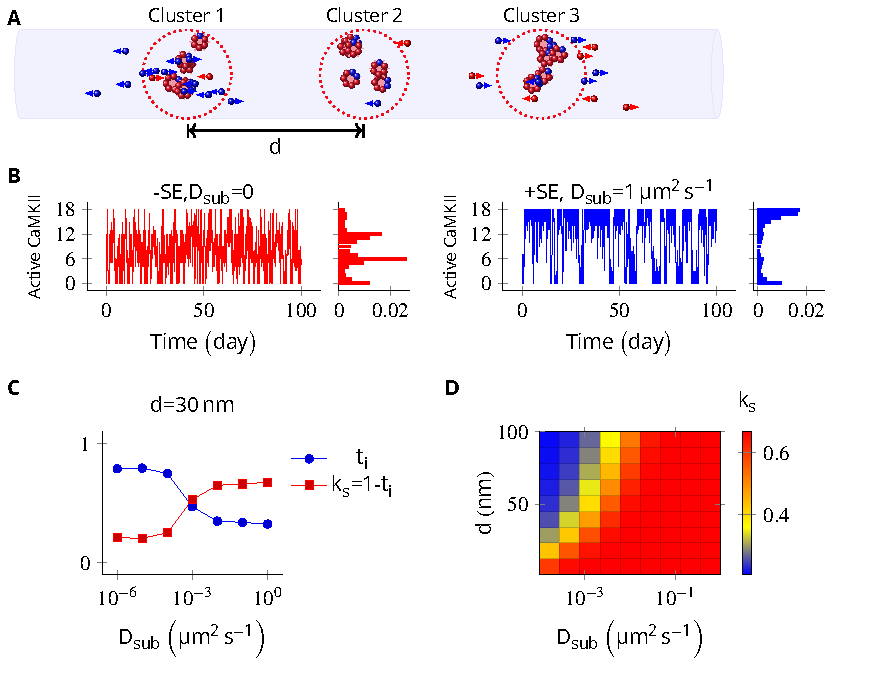
\includegraphics[width=0.95\linewidth]{./PaperFigures/elifeFigure5/figure_sync_150mm.pdf}
    \caption{In the \gls{psd}, subunit exchange synchronizes activity of
        \gls{camkii} clusters. 
        %
        \textbf{(A)} 3 clusters, each of size 6 (i.e.,
        \SUB{N}{CaMKII}=6) separated by distance \(d\) were simulated in a
        cylindrical arena of volume \SI{0.0275}{\micro\meter^3} discretized
        into 3 voxels. \Gls{camkii} subunits are shown as red 
        (unphosphorylated) and blue (phosphorylated) balls. We used 
        %
        \textbf{(B)} (\textbf{left}) Without subunit exchange, all three
        switches flipped independently with low residence time resulting in a
        binomial distribution of states (Bar chart on right, in red). (\textbf{right})
        With subunit exchange, all switches synchronized their activity i.e.,
        they acted as a single bistable switch with larger residence time.
        %
        \textbf{(C)} Strength of synchronization (\SUB{k}{s})
        vs. diffusion constant \SUB{D}{sub} for a system consisting of 3 switches
        each separated from each other by a distance of \SI{30}{\nano \meter}.
        Variable $k_s=1-t_i$ where $t_i$ is the fraction of total time spent by
        the switches in the intermediate states
        x\textsubscript{a}y\textsubscript{n-a}; 1\textless{}a\textless{}n.
        Synchronization is strong if k\textsubscript{s} \textgreater{} 0.4.
        %
        \textbf{(D)} Phase plot of \SUB{k}{s} vs. \SUB{D}{sub} and d. The effect
        of synchronization \SUB{k}{s} due to subunit exchange is strong (red
        region) and robust to changes in \SUB{D}{sub}, and effective for
        inter-cluster distance ($d$) as large as \SI{100}{\nano\meter}. 
        \SUB{D}{PP1}=\SI{0.5}{\micro\meter\squared\per\second} for all
        simulations.
    }\label{fig:sync_spread}
    \figdata{Source and data are available at
    \url{http://github.com/dilawar/SinghAndBhalla_CaMKII_SubunitExchange_2018/tree/master/PaperFigures/elifeFigure5}}
\end{figure}

Next we probed the effect of subunit exchange between spatially separated
\gls{camkii} clusters. We considered \SUB{N}{CaMKII} holoenzymes organized into
three clusters of size \SUB{N}{CaMKII}/3, each separated by a distance \(d\).
This configuration corresponds to cases where receptors and \gls{camkii}
holoenzymes are clustered at the synapse. 

When there is no subunit exchange across voxels (\SUB{D}{sub}=0), these switches
are expected to switch independently like multiple coins flipped together,
resulting in a binomial distribution of activity. The clustered system had 3
relatively stable bistable systems (long residence time, \FIG{validation}E). As
expected, without subunit exchange, activity in this system had a binomial
distribution (\FIG{sync_spread}B, red plot). 

Then we allowed \gls{pp1} and \gls{camkii} subunits to undergo linear diffusion.
We set \SUB{D}{PP1}=\SI{0.5}{\micro\meter\squared\per\second} as before and
varied \SUB{D}{sub} to quantify effect of subunit exchange. Subunit exchange led
to synchronization of switching activity. The population of clustered
\gls{camkii} acted as a single bistable switch (\FIG{sync_spread}B, blue plot).
This effect was strong and robust to variation in \SUB{D}{sub}. Even for a very
small value of \SUB{D}{sub}=\SI{0.01}{\micro\meter\squared\per\second}, we
observed strong synchronization (\FIG{sync_spread}D). The synchronization
disappeared completely for \SUB{D}{sub} less than
\SI{e-4}{\micro\meter\squared\per\second}, and for $d$ greater than
\SI{100}{\nano\meter} (\FIG{sync_spread}D).

Thus, for most physiologically plausible values of diffusion coefficient
\SUB{D}{sub}, subunit exchange causes synchronization of switching activity of
clustered \gls{camkii}.

%%%% Dual decay rate of CaMKII. %%%%%%%%%
\subsection{Subunit exchange may account for the observed dual decay rate of
    CaMKII phosphorylation}\label{subsec:camkii_decay_two_time_course}

Finally, we asked if subunit exchange might account for the complex time-course
of \gls{camkii} dynamics in spine as observed in recent experiments
\citep{chang_camkii_2017}. We designed a simulation to replicate an experiment
where \gls{camkii} was inhibited by a genetically encoded photoactivable
inhibitory peptide after activating \gls{camkii} by glutamate uncaging
\citep{murakoshi_kinetics_2017}. In the spine, \gls{camkii} is more accessible
to phosphatases than in the \gls{psd}, where our previous calculations had been
located. To model the increased availability of phosphatases, we increased the
concentration of \gls{pp1} by an order of magnitude, and increased the volume of
the compartment to match the volume of a typical spine head i.e.,
\SI{0.02}{\cubic\micro\meter} \citep{bartol_nanoconnectomic_2015}. We found that
CaMKII acted as a leaky integrator of the calcium activity with a typical
exponential decay dynamics (\FIG{cytosol_integrator}A). We then enabled the
diffusion of \gls{camkii} subunits
(\SUB{D}{sub}=\SI{1}{\micro\meter\squared\per\second}) and \gls{pp1}
(\SUB{D}{PP1}=\SI{0.5}{\micro\meter\squared\per\second}). These conditions
decreased the rate of dephosphorylation roughly by a factor of 5
(\SI{41.65}{\second} v/s \SI{200.82}{\second}) (\FIG{cytosol_integrator}B). 

\begin{figure}%[t]%[tbh]
    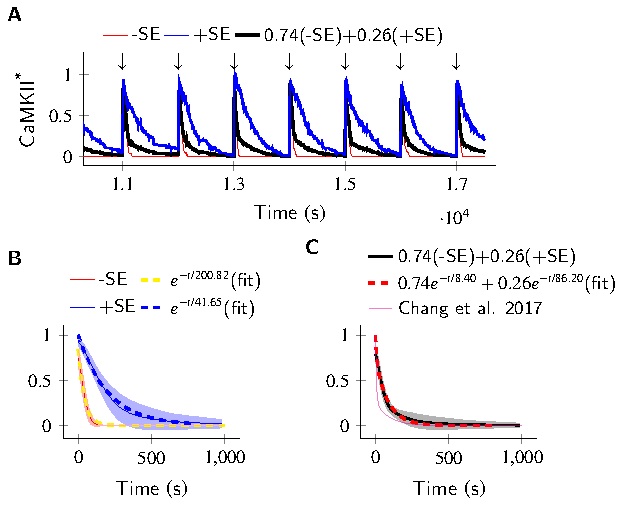
\includegraphics[width=11.4cm]{PaperFigures/elifeFigure6/figure_two_timecourses_114mm.pdf}
    \caption{ In the \gls{pp1} rich spine cytosol, \gls{camkii} acts as a leaky integrator of \gls{ca} 
        activity. As clustered \gls{camkii} population decays much slowly due
        to subunit exchange, a mixed population of clustered and non-clustered \gls{camkii}
        can explain observed two time-constants of \gls{camkii} decay \citep{chang_camkii_2017}.
        \textbf{(A)} Trajectories of \gls{camkii} activity (fraction of all
        \gls{camkii} which are active) are shown when a strong periodic \gls{ca} pulse of \SI{3}{\second}
        duration was applied to the system after every \SI{1000}{\second} ($\downarrow$).
        After the pulse, \gls{ca} levels were brought down to \SI{80}{\nano M}. 
        Three trajectories are shown: without subunit exchange (red), with
        subunit exchange (blue), and a weighed sum of red and blue (74\%
        red + 24\% blue as estimated in \citep{chang_camkii_2017}). 
        \textbf{(B)} Average decay dynamics after the onset of strong \gls{ca} pulse ($\downarrow$). 
        When there is no subunit exchange, \gls{camkii} decays at timescale of
        approximately \SI{41.65}{\second} (red and dashed yellow (fit)). When subunit exchange is enabled, 
        \gls{camkii} decay has larger time-constant of $\SI{200.82}{\second}$
        (blue and dashed blue (fit)). \textbf{(C)} Average dynamics of mixed population
        (black). Fit of mixed population by a double
        exponential i.e. $ae^{-t/\tau_{1}}+(1-a)e^{-t/\tau_{2}}$ for
        $a=0.74$ (dashed red). 
        For a given $a=0.74$ (estimated in \citep{chang_camkii_2017}), our
        estimate of time-constants (\SI{8.4}{\second}, \SI{86.2}{\second}) matches well with experimentally
        estimated time-constants (\SI{6.4}{\second}$\pm$0.7, \SI{92.6}{\second}$\pm$50.7). 
        Shaded areas are the standard deviation. Number of voxels $N_{v}=10$,
        \SUB{D}{sub}=\SI{1}{\micro\meter\squared\per\second},
        \SUB{D}{PP1}=\SI{0.5}{\micro\meter\squared\per\second}.
    }\label{fig:cytosol_integrator}
\figdata{Source and data are available at
\url{http://github.com/dilawar/SinghAndBhalla_CaMKII_SubunitExchange_2018/tree/master/PaperFigures/elifeFigure6}}
\end{figure}

We expected subunit exchange to have a strong effect on the decay activity of
clustered \gls{camkii} in spine cytosol (e.g., \gls{camkii} bound to actin)
because of the proximity of holoenzymes, leading to rapid exchange. Thus, if
there are populations of clustered as well as non-clustered \gls{camkii} in the
spine, we expected that they would exhibit long and short time-courses of
activity decay, respectively. Therefore a mixed population of clustered and
non-clustered \gls{camkii} should decay with two time-constants. Our
simulations supported this prediction. 

In \cite{chang_camkii_2017}, the decay kinetics of \gls{camkii} were obtained by
curve fitting of experimental data. It is given by a double-exponential
function: $F(t)=P_{fast}e^{-t/\tau_{fast}}+P_{slow}e^{-t/\tau_{slow}}$ where
$P_{fast}=0.74, P_{slow}=0.26, \tau_{fast}= 6.4\pm0.7 \si{\second},
\tau_{slow}=92.6 \pm 50.7\si{\second}$ (\FIG{cytosol_integrator}C, magenta). We
used their estimate of $P_{fast}$ and $P_{slow}$ to construct a mixed population
of slow and fast decaying \gls{camkii} (\FIG{cytosol_integrator}A, black) and
estimated a double-exponential function which fits it
(\FIG{cytosol_integrator}C, dashed red). The time-constants obtained
(\SI{8.4}{\second}, \SI{86.2}{\second}) matched well with experimentally
estimated time-constants of (\SI{6.4}{\second}$\pm$0.7,
\SI{92.6}{\second}$\pm$50.7). 

Thus, we suggest that subunit exchange may be a mechanism that leads to
\gls{camkii}$\alpha$ activity decaying with two time-courses in spine 
cytosol.

% DISCUSSION
\section{Discussion}\label{discussion}

Here we have shown that subunit exchange strongly affects the properties of the
CaMKII/PP1 pathway, both in its role as a bistable switch in the PSD and as a
leaky integrator of \gls{ca} activity in spine cytosol. In the PSD, where the
model was tuned to elicit bistable dynamics from clustered \gls{camkii}, subunit
exchange improved the stability of \gls{camkii}/\gls{pp1} switch by
synchronizing the kinase activity across the \gls{psd}
(\FIG{cytosol_integrator}). It also improved active \gls{camkii} tolerance of
PP1 and turnover rate (\FIG{tolerance_pp1} and \FIG{turnover}). In the case
where \gls{camkii} was uniformly distributed in \gls{psd}, subunit exchange
facilitated more rapid activation of \gls{camkii}
(\FIG{subunit_facilitates_spread}B-D)
\citep{stratton_activation-triggered_2014}. These simulation results predict
that a \gls{camkii} mutant lacking subunit exchange would be deficient in switch
stability and slower to be activated by \gls{ca} thereby resulting in degraded
memory retention and deficient learning in memory related behavioural
experiments, respectively.

In the spine head, subunit exchange facilitated integration by prolonging the
decay time-course of kinase activity (\FIG{cytosol_integrator}). The fact that
\gls{camkii} dynamics changed from an integrator to bistable switch as we moved
from spine cytosol (a phosphatase rich environment) to the \gls{psd} (where PP1
is tightly controlled) suggests an interesting sub-compartmentalization of
functions in these microdomains. Furthermore, we observed that the clustering of
\gls{camkii} had important implications for its sustained activity.

Subunit exchange is unlikely to have any impact on neighbouring spines. The mean
escape time of a single \gls{camkii} subunit from a typical spine is between
\SI{8}{\second} to \SI{33}{\second} \citep{holcman_diffusion_2011}. In a real
synapse, this time would be even larger given that \gls{camkii} interacts with
many other molecules. Any phosphorylated subunit is almost certain to be
de-phosphorylated by \gls{pp1} during this time. We therefore predict that the
effects of synchronization are local to each \gls{psd}, where \gls{pp1} is known
to be tightly controlled. Subunit exchange loses its potency in the phosphatase
rich region of the bulk spine head or dendrite. We therefore consider it
unlikely that \gls{camkii} subunit exchange plays any role in intra-spine
information exchange such as synaptic tagging.

\Gls{camkii} is non uniformly distributed in the \gls{psd} where it is mostly
concentrated in a small region of \SI{16}{\nano \meter} to \SI{36}{\nano \meter}
below synaptic cleft \citep{petersen_distribution_2003}. In the \gls{psd},
\gls{camkii} may exist in large clusters given that the \gls{psd} is rich in
\gls{camkii} binding partners. Our study predicts that subunit exchange may
lead to synchronization when \gls{camkii} is clustered, or more rapid activation
by \gls{ca} when it is uniformly distributed. Given that \gls{camkii} can form
clusters with \gls{nmda} receptors, it would be interesting to study the mixed
case where some \gls{camkii} is clustered and the rest is uniformly distributed.
This would require a detailed 3D simulation and is beyond the scope of this 
study.

Finally, we suggest that the existence of diverse multiple time-scales of
\gls{camkii} activity -- bistable and highly stable synchronized bistable in
PSD, slow and fast decaying leaky integrator in spine head -- has important
theoretical implications. A very plastic synapse is good at registering activity
dependent changes (learning) but poor at retaining old memories. On the other
hand, a rigid synapse is good at retaining old memories but is not efficient at
learning. A theoretical meta-model which sought to strike a balance between
these two competing demands requires that a diversity of timescales must exist
at the synapse \citep{benna_computational_2016} for optimum performance. In
this model, complex synapses with state variables with diverse time-scales are
shown to form a memory network in which storage capacity scales linearly with
the number of synapses, and memory decay follows \(1/\sqrt{t}\) --- a power-law
supported by psychological studies \citep{wixted_form_1991}. This model requires
the memory trace to be first stored in a fast variable and then progressively
and efficiently transferred to slower variables. Our study suggests a concrete
mechanism for such a process. Here, the \gls{ca} concentration in the PSD can be
mapped to the fastest variable. The \gls{camkii} integrator in the cytosol could
represent the second slower variable to which the trace is transferred from
\gls{ca}. Further, the state information is transferred to the third slower
\gls{camkii} bistable switch. The dynamics of \gls{camkii} in the PSD forms an
even slower bistable variable for longer retention of the memory trace. It is
possible that memory is transferred from here to even slower variables, such as
sustained receptor insertion \citep{hayer_molecular_2005}, PKM-$\zeta$
activation \citep{sacktor_memory_2012}, or local protein synthesis
\citep{aslam_translational_2009}.

% MATERIALS AND METHODS
\section{Methods and Materials}{\label{sec:materials_and_methods} 

We extended Miller and Zhabotinksy (MZ model) \citep{miller_stability_2005} to
incorporate \emph{subunit exchange} and diffusion. We assume that vertical
dimers are inserted and released together \citep{bhattacharyya_molecular_2016}.
We also assume that both subunits of a vertical dimer phosphorylate and
de-phosphorylate together. Under this assumption, we can treat the \gls{camkii}
ring as the proxy for the \gls{camkii} holoenzyme and the subunit as the proxy
for the \gls{camkii} dimer. Without this assumption, the simulation cost of the
increased complexity would be very significant. The qualitative aspect of model
behaviour will be the same with or without this assumption. 

In our model, a \gls{camkii} ring with $n$ subunits ($n$=6 or 7) can exist
in 15 different states enumerated as $x_{a}y_{n-a}$ for $0 \le a \le n$ where
$x$ and $y$ represents un-phosphorylated and phosphorylated subunits
respectively. We ignore all rotational permutations and kinetically unlikely
cases where there are discontiguous phosphorylated subunits in the ring. We
assumed that the phosphorylation of neighbouring subunit proceeds clockwise.

\subsection{\SUP{Ca}{2+} background activity ($\epsilon$)}\label{subsec:calcium_background}

We assumed the resting \gls{ca} level in spine to be \SI{80}{\nano M}
\citep{berridge_neuronal_1998}. In \gls{mz} model, Miller \textit{et al.}
assumed that \gls{ca} entry through \gls{nmda} receptors can be approximated by
a Poisson train with an average rate of \SI{0.5}{Hz}. Since, on average,
$\sim$0.5 \gls{nmda} receptor opens \citep{nimchinsky_number_2004} upon
pre-synaptic stimulation, we reduced the frequency of NMDA opening events to
\SI{0.25}{Hz}. We used a periodic pulse with time-period of \SI{4}{\second} and
duty cycle of 50\%. To model NMDA activity in \SI{2}{\second} long \texttt{ON}
period of our \SI{4}{\second} long periodic pulse, we sampled from a uniform
distribution with median of \SI{120}{\nano M} (50\% change, on average) and
range of \SI{40}{\nano M} (\FIG{validation}C). This distribution is informed by
figure 2B,C from \citep{nimchinsky_number_2004}.

We did not consider decay dynamics of \gls{ca} influx through \gls{nmda} channel
since including the timescale of decay (roughly \SI{100}{\milli\second}) would
have made simulation very slow. The effect of ignoring decay dynamics are
expected to be negligible given the time-scale of \gls{camkii} activation is
much larger than the time course of \gls{ca} decay dynamics. Furthermore, we did
not consider contributions to background \gls{ca} fluctuations by other
channels. This background activity is represented by $\epsilon$ in other
figures.

\subsection{Phosphorylation and dephosphorylation of CaMKII ring}
\label{phosphorylation-and-dephosphorylation-of-ring} 

The activation of \gls{camkii} follows the same dynamics as in \gls{mz} model
(\EQ{phospho}). In this paper, by phosphorylation/activation of a \gls{camkii}
subunit or a holoenzyme, we mean phosphorylation at \SUP{Thr}{286}. The first
step in \gls{camkii} activation requires simultaneous binding of two \gls{cacam}
to the two adjacent subunits of \gls{camkii}. Once a subunit is phosphorylated
(\SUP{Thr}{286}), it catalyzes phosphorylation of it's neighbour
(\emph{auto-phosphorylation}) which requires binding of only one \gls{cacam}.
Therefore, further phosphorylation proceeds at much faster rate.  The
phosphorylation of \gls{camkii} (\SUP{Thr}{286}) is given by \EQ{phospho}
\citep{bradshaw_ultrasensitive_2003,miller_stability_2005}.

\begin{equation}\label{eq:phospho}
    \newcommand\CaHILL{\ensuremath{\frac{Ca^{2+}}{K_{H1}}}}
    \newcommand\VONE{k_1 \left[\frac{H^3}{1+H^3}\right]^2}
    \newcommand\VTWO{k_1\frac{H^3}{1+H ^3}}
\begin{gathered}
    x_ay_{n-a} \xrightarrow{v_1} x_{a-1}y_{n-a+1} \xrightarrow{v_2} x_{a-2}y_{n-a+2} \\
    v_1 = \VONE,\, v_2 =\VTWO,\,\text{where}\; H=\CaHILL
\end{gathered}
\end{equation} where $n=6\;\text{or}\;7$ for $1\le a \le n$;
$k_1=\SI{1.5}{\per\second}$ \citep{hanson_dual_1994}, and
$k_{H1}=\SI{0.7}{\micro M}$ \citep{koninck_sensitivity_1998,miller_stability_2005}.
At resting \gls{ca} concentration of \SI{100}{\nano M}, $v_1=\SI{1.27e-5}{\per\second}$ and
$v_2=\SI{4.36e-3}{\per\second}$ (i.e., ${v_2}/{v_1}\approx 343$).

Once fully phosphorylated, \gls{camkii} moves to \gls{psd} where it binds to
\gls{nmda} receptor. Upon binding, it is no longer accessible other phosphatases
save \gls{pp1}.

The dephosphorylation of the \gls{camkii} ring, and the subunit is given by
\EQ{dephosphorylation}.

\begin{equation}\label{eq:dephosphorylation} 
    \begin{gathered} 
        PP1 + x_ay_{n-a} \xrightleftharpoons[k^-]{k^+} PP1.x_ay_{n-a} 
            \xrightarrow{k_2} PP1 + x_{a+1}y_{n-a-1} \\ 
        PP1 + x \xrightleftharpoons[k^-]{k^+} PP1.x \xrightarrow{k_2} PP1 + y 
    \end{gathered}
\end{equation}

\noindent where $n=6\;\text{or}\;7$, and $1\le a \le n$. Following
\cite{miller_stability_2005}, we also assumed $k^-=0$. This gave us
$k^+=\frac{k_2}{k_M}=\SI{1}{\per\micro M\per\second}$. We could not find any
experimental estimate of $k_M$ in recent literature, therefore we used the same
value of $k_M$ used in the \gls{mz} model \citep{miller_stability_2005}.

\subsection{Subunit exchange}\label{subunit exchange} 

Since \gls{camkii} ring consists of either 6 or 7 subunits exists in our model,
any ring with 6 subunits cannot lose a subunit, and a ring with 7 subunits
cannot gain a subunit. The reactions which result in either gain or lose of a
subunit are given by \EQ{losegainx} where $0\le a \le 6\text{ or }7$.

\begin{equation}\label{eq:losegainx}
    \begin{gathered}
    x_ay_{7-a} + x \xrightleftharpoons[k^-_x]{k^+_x} x_{a+1}y_{6-a} \\
    x_ay_{6-a} + y \xrightleftharpoons[k^-_y]{k^+_y} x_{a}y_{7-a}
    \end{gathered}
\end{equation}

The values of $k_x^+$, $k_x^-$, $k_y^+$, and $k_y^-$ are not available in the
literature that we are aware of. We used the data in
\cite{stratton_activation-triggered_2014} to estimate the possible timescale of
subunit exchange rate. \cite{bhattacharyya_molecular_2016} speculate that upon
activation, the hub of holoenzyme becomes less stable and more likely to open up
and lose a subunit i.e., active holoenzyme loses a subunit faster. Therefore, we
maintained the following ratio \(k_x^- \approx 10 k_x^+ N_{\text{CaMKII}}\) and
\(k_y^- \approx 10 k_y^+ N_{\text{CaMKII}}\) in all simulations where
\SUB{N}{CaMKII} is the number of holoenzymes in the system.

% Estimation of subunit exchange rate.
\subsubsection{Estimation of subunit exchange rate}\label{subsec:estimate_exchange_rate}

To estimate reaction rates of \EQ{losegainx}, we modeled the "single molecule
assay" used in \cite{stratton_activation-triggered_2014}. In this assay, two
distinct populations of \gls{camkii} labelled by either green or red
fluorophores were mixed together. The holoenzymes were not free to move but they
could release subunits which could move freely. A green holoenzyme may pick up a
red subunit and vice versa thereby giving rise to a mixed colored population.
The readout from this assay is the ``colocalization'' which is the fraction of
total holoenzymes containing subunits of both colors.

In our model of this assay, a \gls{camkii} holoenzyme is represented by
$R_aG_{n-a}$ where $R$ and $G$ represent a red and a green subunit in the
holoenzyme respectively, and $n=6\;\text{or}\;7$. The green population consists
of holoenzymes with only green subunits (i.e., $R_0G_6$ and $R_0G_7$) and the
red population has holoenzymes with all red subunits (i.e., $R_6G_0$ or
$R_7G_0$). We assume that each color population has equal number of dodecameric
(n=6$\times$2) and tetradecameric (n=7$\times$2) holoenzymes. Upon mixing red and green
populations, the following reactions take place.

\begin{equation}\label{eq:mixing_assay}
    \begin{gathered}
        R_aG_b \xrightleftharpoons[r_g]{r_l} R_{a-1}G_b + R 
        \quad \text{for all}\; a>0,b\ge 0\; \text{s.t.}\; a+b=6 \\
        R_aG_b \xrightleftharpoons[r_g]{r_l} R_{a}G_{b-1} + G 
        \quad \text{for all}\; a\ge 0,b> 0\; \text{s.t.}\; a+b=7
    \end{gathered}
\end{equation}

The value of colocalization is equal to the percentage of all holoenzymes
containing at least one red and one green subunit i.e. $\frac{\sum_{a\ge 1, b
\ge 1} [R_aG_b]}{ \sum_{a\ge0,b \ge 0}[R_aG_b]}$. The dynamics of colocalization
was fit by $100(1-e^{-t/\tau})$. We first computed $\tau$ for experimental data
when [CaMKII]=\SI{8}{\micro M} (\FIG{estimate_of_exchange_rate}A). This served
as the baseline for further analysis.

Next we explored the space of $r_l$ and $r_g$ for which the time constant $\tau$
of colocalization dynamics matched well with the baseline case (ie., $\tau$ for
these trajectories were $\tau_{\text{[CaMKII]=8}} \pm 20\%$
(\FIG{estimate_of_exchange_rate}B, black dots)}.  From these values, we chose a
combination of $r_g$ and $r_l$ which best explained the concentration dependant
changes in the rate of colocalization (\FIG{estimate_of_exchange_rate}D). When
compared with the data from \cite{stratton_activation-triggered_2014}, the time
scale of colocalization and the concentration dependant decrease in the rate of
colocalization compared reasonably well for $r_l$ and $r_g$ ie.,
$\tau=\SI{49.1}{\min}$ (data) vs $\tau=\SI{21.0}{min}$ (simulation) when
[CaMKII]=\SI{8}{\micro M} and $\tau=\SI{119.0}{min}$ (data) vs
$\tau=\SI{150.0}{min}$ (simulation) when [CaMKII]=\SI{1}{\micro M}, and,
$\frac{d\tau}{d\text{[CaMKII]}}=\SI{-10.06}{min\per\micro M}$ (data) vs
$\frac{d\tau}{d\text{[CaMKII]}}=\SI{-18.05}{min\per\micro M}$ (simulation)
(\FIG{estimate_of_exchange_rate}D). Note that we do not model effect of
diffusion, labelling efficiency, and experimental errors in readout mechanism.
Our values of $k_x^+, k_y^+, k_x^-, k_y^-$ used in \EQ{losegainx} are close to
estimated values of $r_g$ and $r_l$ (red cross v/s black dots in
\FIG{estimate_of_exchange_rate}B). Note that $r_g$ and $r_l$ are proxies for
$k_x^+,k_y^+$ and $k_x^-, k_y^-$ respectively.

\begin{figure}[ht!]
    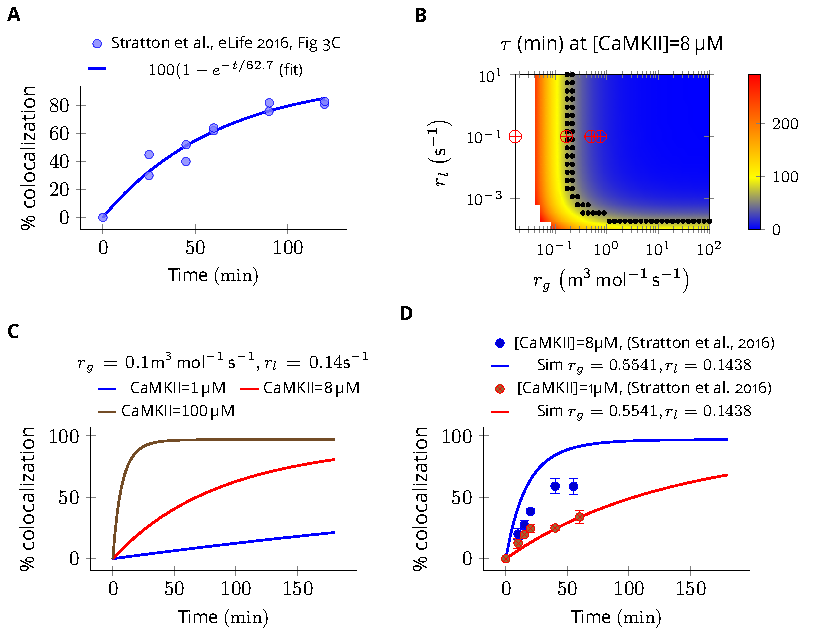
\includegraphics[width=0.95\linewidth]{./PaperFigures/elifeFigure8/figure_exchange_rate.pdf}
    \caption{Rough estimation of subunit exchange rate by fitting experimental
        data to a model of "single molecule assay" \cite{stratton_activation-triggered_2014}. 
        %
        \textbf{(A)} Colocalization dynamics as reported in 
        \cite{stratton_activation-triggered_2014} (all data scraped from figures) at
        \gls{camkii}=\SI{8}{\micro M} (blue dots). Solid blue line shows a best
        fit $100(1-e^{-t/\tau})$ with $\tau$=\SI{62.7}{min}. 
        %
        \textbf{(B)} Phase plot of $\tau$ of colocalization trajectories generated 
        for various values of $r_g$ and $r_l$ (\EQ{mixing_assay}). Black dots show values
        of $r_g$ and $r_l$ for which $\tau=62.7\pm 20\%$ (S.E.M.). Red
        $\oplus$ marks show the values of rate constants (\EQ{losegainx}) 
        used in this study at various volume and \SUB{N}{CaMKII}. 
        %
        \textbf{(C)} For the fixed values of $r_g$ and $r_l$, three trajectories 
        are shown at different \gls{camkii} concentrations. As seen in experimental data
        , rate of colocalization increases with increasing \gls{camkii} concentration. 
        %
        \textbf{(D)} For typical values of exchange rates used in this paper, we plotted
        simulation results (solid lines) with experimental values (dots) and their best
        exponential fit (dashed lines). The ${d\tau}/{d\left[\text{\tiny CaMKII}\right]}$ 
        was \SI{-10.06}{min \per \micro M} (data) and \SI{-18.54}{min\per\micro
        M} (simulation).
    }\label{fig:estimate_of_exchange_rate}
\end{figure}

Thus we are confident that rate parameters used in \EQ{losegainx} in our model
are likely to be within the physiologically relevant range.

\subsection{PP1 deactivation}\label{subsec:pp1_deactivation} 

In the \gls{psd}, \gls{pp1} is the primary -- and perhaps only -- phosphatase
known to dephosphorylate \gls{camkii} \citep{strack_translocation_1997}. We
followed \gls{mz} model for \EQ{i1pandpp1} where \gls{i1} inactivates \gls{pp1}. 
\Gls{i1p} renders \gls{pp1} inactive by forming \gls{i1ppp1}. 

\begin{equation}\label{eq:i1pandpp1}
    \begin{gathered}
        PP1 + I1P \xrightleftharpoons[k_4]{k_3} I1P.PP1 \\
        I1P = I1 \frac{v_{PKA}}{v_{CaN}} 
            \frac{1+\left(\frac{Ca}{k_{H2}}\right)^3}{\left(\frac{Ca}{k_{H2}}\right)^3}
    \end{gathered}
\end{equation}

\noindent where $k_3=\SI{100}{\per\micro M\per\second}$,
$k_4=\SI{0.1}{\per\second}$ \citep{endo_multiple_1996}, and $v_{PKA}/v_{CaN}=1$
\citep{miller_stability_2005}.

\subsection{Turnover}\label{turnover}

The turnover of \gls{camkii} is a continuous process given by \EQ{turnover} with rate
$v_{t}=\SI{30}{\per\hour}$ \citep{ehlers_activity_2003}.

\begin{equation} \label{eq:turnover}
    \begin{gathered}
        x_ay_{6-a} \xrightarrow{v_t} x_6y_0\; \text{for}\; 6\ge a\ge 1 \\
        x_ay_{7-a} \xrightarrow{v_t} x_7y_0\; \text{for}\; 7\ge a\ge 1
    \end{gathered}
\end{equation}

\subsection{Diffusion and simulation method}\label{subsec:simulator}

Diffusion is implemented as cross voxel ``jump'' reaction. Diffusion of a
species X with diffusion-coefficient \SUB{D}{X} between voxel A and B separated
by distance $h$ is modelled by reaction $X_A \xrightleftharpoons[k]{k} X_B$
where \( k={D_X}/{h^2}\), and \([X_A]=[X_B]=[X]/2 \)
\citep{erban_practical_2007}. Based on our own numerical results (Appendix 1, \autoref{fig:suppl_reac_rdme}) and
other studies \citep{isaacson_reaction-diffusion_2009,erban_stochastic_2009}, we
are confident that \( h \ge 10h_{crit}\) where
\(h_{crit}=\frac{k^+}{D_{PP1}+D_{sub}}\) is a good value. We have \( h_{crit} \le \SI{3.2}{\nano\meter} \)
whenever $D_{PP1}+D_{sub}\ge\SI{0.5}{\micro\meter\squared\per\second}$. For all
simulations presented in main text, we maintain $h\ge h_{crit}$. For a case
where $h$ is smaller than $h_{crit}$ in some trajectories see
\FIGSUPP[subunit_facilitates_spread]{diffusion_reduces_pp1_potency}. 

All simulations were performed using Stochastic solver (Gillespie method)
available in MOOSE simulator (\url{https://moose.ncbs.res.in}, version 3.1.4)
\citep{ray_pymoose:_2008}. This model is available
at \url{https://github.com/dilawar/SinghAndBhalla_CaMKII_SubunitExchange_2018}.
Table of parameters can be found in SI (\TABLE{si:parameters}).

\subsection{Method Validation}

To validate our implementation of diffusion, we compared trajectories of two
systems: one in a single `well-mixed' cylinder with with parameters tuned to
elicit bistable behaviour (henceforth, we call it reference bistable), and other
in a discretized cylinder as described above. We expect the later to converge to
reference bistable system. 

We put 6 \gls{camkii} holoenzymes in a cylinder of length \SI{180}{\nano\meter}
discretized into 6 voxels, separated by a distance of \SI{30}{\nano\meter}. The
long-term behaviour of discretized system was most sensitive to \SUB{D}{PP1}
(\FIG{method_validation}B) and almost independent of \SUB{D}{sub}
(\FIG{method_validation}A). The discretized system converges to reference
bistable (\FIG{method_validation}C, black dots). The sensitivity of \SUB{D}{PP1}
is due to the fact that long-time average potency of \gls{pp1} reduced with
increased \SUB{D}{PP1}
(\FIGSUPP[method_validation]{diffusion_reduces_pp1_potency}) which led to
decreased average \gls{pp1} activity and hence increased average \gls{camkii}
activity (\FIG{method_validation}C, red region). This effect is not entirely due
to numerical errors as shown in \FIGSUPP[method_validation]{diffusion_reduces_pp1_potency}. 

\begin{figure}[ht!]
    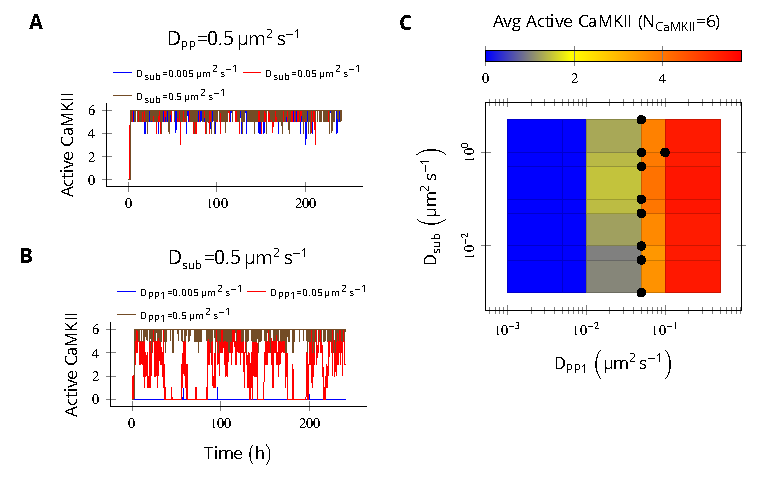
\includegraphics[width=12cm]{./PaperFigures/elifeFigure7/figure_su_long_term_effect.pdf}
    \caption{Method validation. \SUB{N}{CaMKII}=6 holoenzymes as described in
        the \FIG{subunit_facilitates_spread} are simulated in a cylinderical arena divided
        into 6 voxels separated by \SI{30}{\nano\meter}. Basal \gls{ca} label
        fixed to \SI{100}{\nano M}+$\epsilon$. Another system with same
        parameter set was simulated in a single `well-mixed' cylinder of 
        same length and volume known to elicit bistable
        behaviour (henceforth reference bistable system, data not shown). 
        \textbf{(A)} For fixed \SUB{D}{PP1}=\SI{0.5}{\micro\meter\squared\per\second}, varying
        \SUB{D}{sub} does not affect average \gls{camkii} activity. 
        \textbf{(B)} On the other hand, for fixed
        \SUB{D}{sub}=\SI{0.5}{\micro\meter\squared\per\second} , increasing
        \SUB{D}{PP1}, increases average \gls{camkii} activity. We see a bistable
        trajectory (red) which is similar to the behaviour or reference bistable
        system (data not shown). \textbf{(C)} Phase plot shows the discretized
        system converges to reference bistable system (black dots). Long time
        average \Gls{camkii} activity (simulation time=10 days) is independent of 
        \SUB{D}{sub}, and only depends on \SUB{D}{PP1}. Black dots represent bistable
        configurations with at least 4 transitions observed in 10 days long
        simulation. Thus discretized system converges to reference bistable system.
    }\label{fig:method_validation} 

    % suppl
    \figsupp[\gls{pp1} potency reduces as \SUB{D}{PP1} increases.]{CaMKII/PP1
        system was simulated in a cylinderical arena discretized into 6 voxels 
        of equal volume separated by distance \(h\)=\SI{30}{\nano\meter}.
        %
        \textbf{(A)} \textbf{(above)} For each voxel, trajectory of active \gls{pp1} v/s time
        is plotted in blue. \textbf{(below)} Cross-correlation matrix (Pearson
        product-moment correlation coefficient, using \texttt{numpy.corrcoef}
        function). 
        % B
        \textbf{(B,C)} Same as \textbf{A} but with different value of
        \SUB{D}{PP1}, \SI{0.001}{\micro\meter\squared\per\second} and
        \SI{0.1}{\micro\meter\squared\per\second} respectively. \gls{pp1}
        activity reduces in all voxels with increased \SUB{D}{PP1}. The
        correlation of \gls{pp1} activity among voxels does not improve with
        increased \SUB{D}{PP1} therefore non-linear distribution of \gls{pp1} in
        voxels is unlikely to be a significant contributor to the observed loss
        of \gls{pp1} potency. 
        %
        \textbf{(D)} \gls{pp1} activity decreased with increased \SUB{D}{PP1} 
        but remained independent of diffusion coefficient
        of subunit (\SUB{D}{sub}). On y-axis, \gls{pp1} activity is measured as
        ratio of sum of number of all active \gls{pp1} in all voxels during the
        simulation divided by the simulation time in hours. On top, dotted blue
        line (labeled \textcolor{blue}{\SUB{D}{PP1}=0}) represents the case
        where \gls{pp1} was not allowed to diffuse. At bottom, dotted blue line
        (labeled \textcolor{blue}{1-voxel}) shows the case where the cylinder
        consists only of 1 voxel and diffusion is instantaneous i.e., it is a
        well-mixed system. As expected, as \SUB{D}{PP1} increased, the 6 voxels
        system converged to a well-mixed system of 1 voxel of 6x volume. Note
        that a similar effect is seen for a range of \SUB{D}{sub}, including
        \SUB{D}{sub}=\SI{5}{\micro\meter\squared\per\second}, for which
        $h_{crit}=\SI{0.33}{\nano\meter}$, satisfying the condition \(h\gg
        h_{crit}\) \citep{isaacson_reaction-diffusion_2009,erban_stochastic_2009}.
        (Also see Appendix 1, \autoref{fig:suppl_reac_rdme} and
        \nameref{sec:diff_as_gillespie}) Thus we do not expect that this is a
        numerical artifact due to our use of cross-voxel jump reactions to
        approximate diffusion.
    }{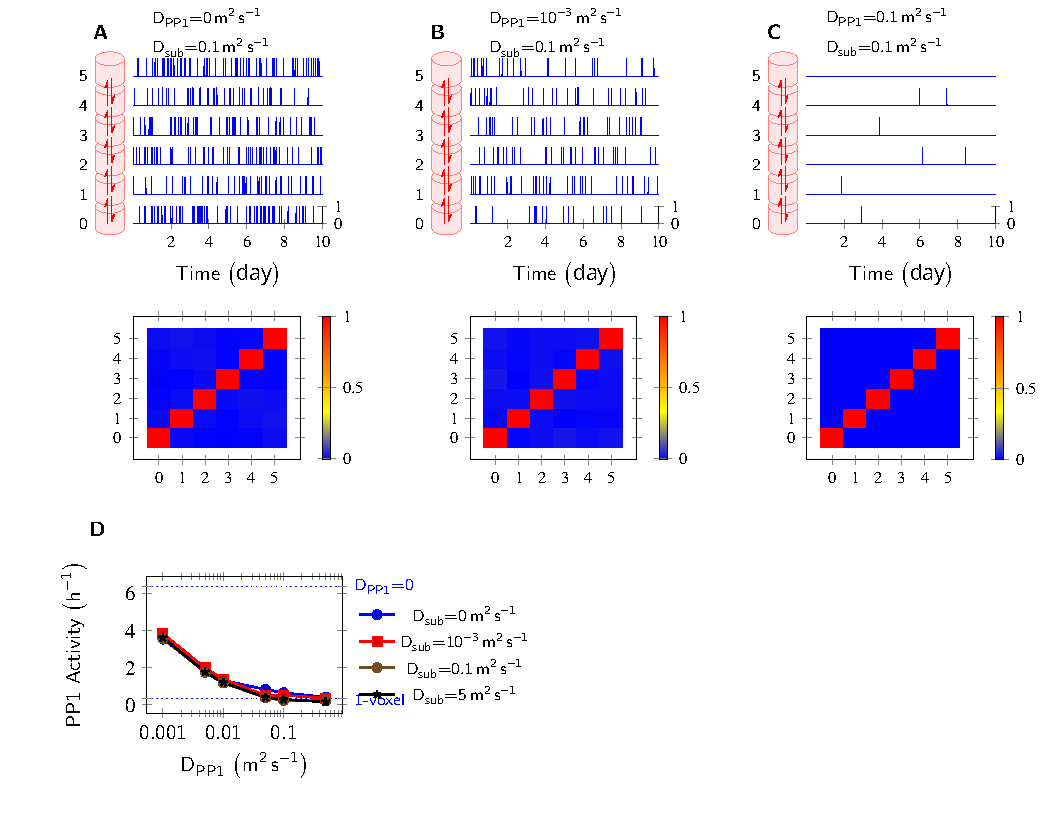
\includegraphics[width=\linewidth]{./PaperFigures/suppl/figure_pp1_profile.pdf}}
    \label{figsupp:diffusion_reduces_pp1_potency} \end{figure}

\subsection{Table of parameters} 
\TABLE{si:parameters} summarizes parameters of our model.

\begin{singlespace}
\begin{table}[t] %[hbt]
    \caption{Table of parameters used in model.}\label{tab:si:parameters}
    \begin{tabularx}{\linewidth}{p{15mm} p{0.4\linewidth} X X}
        \toprule
        \textbf{Symbol} & \textbf{Parameter} & \textbf{Value} & \textbf{Ref}\\
        \midrule
        V\textsubscript{Spine} & Volume of Spine & 1 to \SI{5e-20}{\cubic \meter} & \citep{bartol_nanoconnectomic_2015}\\ 
        V\textsubscript{PSD} & Volume of PSD (Thickness 
                                \texttildelow\SI{100}{\nano \meter}. 
                                Surface area \texttildelow\SI{0.05}{\cubic\micro\meter}) 
                             & 1 to \SI{5e-21}{\cubic \meter} 
                             & \citep{farley_structure_2015,bartol_nanoconnectomic_2015}\\
        N\textsubscript{CaMKII} & Total CaMKII holoenzymes in PSD/Spine & 100$\pm$18 & \citep{farley_structure_2015}\\
        N\textsubscript{PP1} & Total PP1 in PSD & 4 to 20\(\times\)N\textsubscript{CaMKII} & This paper\\
                             & Total PP1 in Spine & 10 to 100\(\times\)N\textsubscript{CaMKII} & This paper\\
        I1 & Concentration of free
        I1 & \SI{0.1}{\micro M} & \citep{miller_stability_2005}\\
        V\textsubscript{CaN} & Activity of calcineurin divided by its Michaelis
        constant & \SI{1.0}{\per \second} & \citep{miller_stability_2005}\\
        V\textsubscript{CaM} & Activity of PKA divided by its Michaelis
        constant & \SI{1.0}{\per \second} & \citep{miller_stability_2005}\\
        K\textsubscript{M} & The Michaelis constant of
        PP1 & \SI{10}{\micro M} & 0.4 to 20 \si{\micro M} \citep{zhabotinsky_bistability_2000}\\
        K\textsubscript{H1} & Hill constant of CaMKII (\gls{ca})
        activation) & \SI{0.7}{\micro M} & \citep{koninck_sensitivity_1998}\\
        n\textsubscript{H1} & Hill coefficient of CaMKII (\gls{ca})
        activation) & 3 & \citep{stemmer_dual_1994}\\
        K\textsubscript{H2} & Hill constant of calcineurin (\gls{ca}
        activation) & \SI{0.3}{\micro M} & \citep{stemmer_dual_1994}\\
        n\textsubscript{H2} & Hill constant of calcineurin
        (\gls{ca} activation) & 3 & \citep{stemmer_dual_1994}\\
        k\textsubscript{1} & The catalytic constant of
        autophosphorylation & \SI{1.5}{\per\second} & \citep{hanson_dual_1994}\\
        k\textsubscript{2} & The catalytic constant of protein
        phosphotase & \SI{10}{\per\second} & \citep{bradshaw_ultrasensitive_2003,ichikawa_interactions_1996}\\
        k\textsubscript{3} & The association rate constant of PP1.I1P
        complex & \SI{100}{\micro M^{-1}\second^{-1}} &
        \citep{endo_multiple_1996,miller_stability_2005}\\
        k\textsubscript{4} & The dissociation rate constant of PP1.I1P
        complex & \SI{0.1}{\second^{-1}} & \citep{endo_multiple_1996,miller_stability_2005}\\
        k\textsubscript{x}\textsuperscript{+} & The rate of adding 
        unphosphorylated subunit x & \SI{1}{\per\second\per \SUB{N}{CaMKII}} & This paper\\
        k\textsubscript{y}\textsuperscript{+} & The rate of adding
        phosphorylated subunit y & \SI{1}{\per\second\per\SUB{N}{CaMKII}} & This paper\\
        k\textsubscript{x}\textsuperscript{-} & The rate of losing
        unphosphorylated subunit x & \SI{0.1}{\per \second} & This paper\\
        k\textsubscript{y}\textsuperscript{-} & The rate of losing
        phosphorylated subunit y & \SI{0.1}{\per \second} & This paper\\
        v\textsubscript{t} & Turnover rate of CaMKII & \SI{30}{\hour^{-1}} &
        \citep{ehlers_activity_2003,miller_stability_2005}\\
        D\textsubscript{PP1} & Diffusion coefficient of \gls{pp1} & 
        \SI{0.5}{\micro\meter\squared\per\second} & This paper and
        \citep{harvey_spread_2008}\\
        D\textsubscript{sub} & Diffusion coefficient of \gls{camkii} subunits & 
        \SI{e-5}-\SI{10}{\micro\meter\squared\per\second} & This paper \\
        \bottomrule
    \end{tabularx}
\end{table}
\end{singlespace}


%%  ACKNOWLEDGEMENTS %%
\section{Acknowledgements}
We'd like to thank Marcus Benna, Stefano Fusi and Moitrayee Bhattacharyya for
discussions related to their work, Mukund Thattai for useful discussions on the
stochastic reaction diffusion methods, and Bhanu Priya for useful comments on
the manuscript. This work was funded by NCBS/TIFR and SERB JC Bose fellowship
\texttt{SB/S2/JCB-023/2016} to USB.

\bibliography{bibliography} 

\appendix
\begin{appendixbox}

% alternative row
\subsection*{Stochastic diffusion using cross-voxel reactions}\label{sec:diff_as_gillespie}

To implement diffusion of a molecule in a linear arena of volume $V$, we
construct a cylindrical compartment of volumne $V$ with length $L$ and radius
$r$. The cylinder is divided into $n$ \emph{well-mixed} voxels of length $h$
($h=L/n$) i.e., within a voxel, diffusion is instantaneous.

Diffusion across these voxels is implemented as cross-voxel reactions in which a
molecule \emph{jump} to its neighbouring voxels with a rate constant $k$ which
is a function of diffusion coefficient $D$ and length of voxel $h$. Accuracy of
this methods increases as $h$ decreases and converges to analytical solution for
$\lim_{h \to 0}$. The cost of simulation increases as $h$ decreases.

For example, assume that molecule A with diffusion coefficient of $D_A$ is put
into a cylinder. We divide the entire cylinderical volume into $n$ voxels. We
uniformly distribute all molecules of A into these $n$ voxels. Any molecule from
voxel $i$ (labelled $A_i$) can only jump to neighbouring voxel $i+1$ or $i-1$
with rate $k_D^A$. This process is described by following chemical reactions
(\EQ{stoch_diff}).

\begin{equation}
\begin{gathered}
    \ldots A_{i-1} \xrightleftharpoons[k_D^A]{k_D^A} A_{i}
    \xrightleftharpoons[k_D^A]{k_D^A} A_{i+1} \ldots
\end{gathered}
\label{eq:stoch_diff}
\end{equation}


%% METHOD: Stochastic diffusion.
\subsection*{Stochastic diffusion with bimolecular reaction}\label{subsec:rdme}

Consider a cylindrical arena with a simple bimolecular reaction $A+B \rightarrow \phi$.
Both A and B diffuse while $\phi$ does not. In our model, this reaction
resembles dephosphorylation of subunit or \gls{camkii} holoenzyme by \gls{pp1} .
If we divide the cylinder into $n$ voxels labelled 1, 2, $\ldots$, $n$, then we
have following resultant chemical system.

\begin{equation}
    \begin{gathered}
        A_1 + B_1 \xrightarrow{k} \phi_1 \\
        A_2 + B_2 \xrightarrow{k} \phi_2 \\
        \vdots \\
        A_n + B_n \xrightarrow{k} \phi_n \\
        A_1 \xrightleftharpoons[k_D^A]{k_D^A} A_2 ,\, A_2 \xrightleftharpoons[k_D^A]{k_D^A} A_3 
            ,\, \ldots,\, A_{n-1} \xrightleftharpoons[k_D^A]{k_D^A} A_n \\ 
        B_1 \xrightleftharpoons[k_D^B]{k_D^B} B_2 ,\, 
            B_2 \xrightleftharpoons[k_D^B]{k_D^B} B_3 ,\, 
            \ldots,\, B_{n-1} \xrightleftharpoons[k_D^B]{k_D^B} B_n \\ 
    \end{gathered}
    \label{eq:discrete}
\end{equation} where $k_D^A=\frac{D_A}{h^2}$ and $k_D^B=\frac{D_B}{h^2}$ and
$[A_1]=[A_2]=\ldots=[A_n]=[A]$, $[B_1]=[B_2]=\ldots=[B_n]=[B]$ where $[X]$ is
concentration of X.

\begin{center}
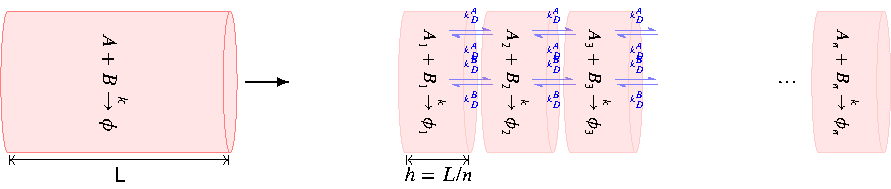
\includegraphics[width=0.8\linewidth]{./PaperFigures/suppl/figure_diff.pdf}
\captionof{figure}{Summary of the stochastic reaction diffusion method employed.}
\end{center}

For a bimolecular system described by \EQ{discrete} when solved using Gillespie
algorithm, as $h$ decreases, the accuracy of solution increases first after
which it starts decreasing. This is because with decreasing $h$, the diffusion
component becomes more precise but we start losing reaction events
\citep{gardiner_correlations_1976}. Analytical methods suggests a lower bound on
$h$, namely $h\gg \frac{k}{D_A+D_B}$ below which errors in the solution are
large \citep{isaacson_reaction-diffusion_2009}. A numerical study
\citep{erban_stochastic_2009} suggests that $h\ge 10\frac{k}{D_A+D_B}$ is a good
value which keeps errors less than 1\% in the distributions of trajectory.

Here, we simulate the system and estimate relative errors for various values of
diffusion coefficient (Appendix 1, \autoref{fig:suppl_reac_rdme}).

\begin{center}
    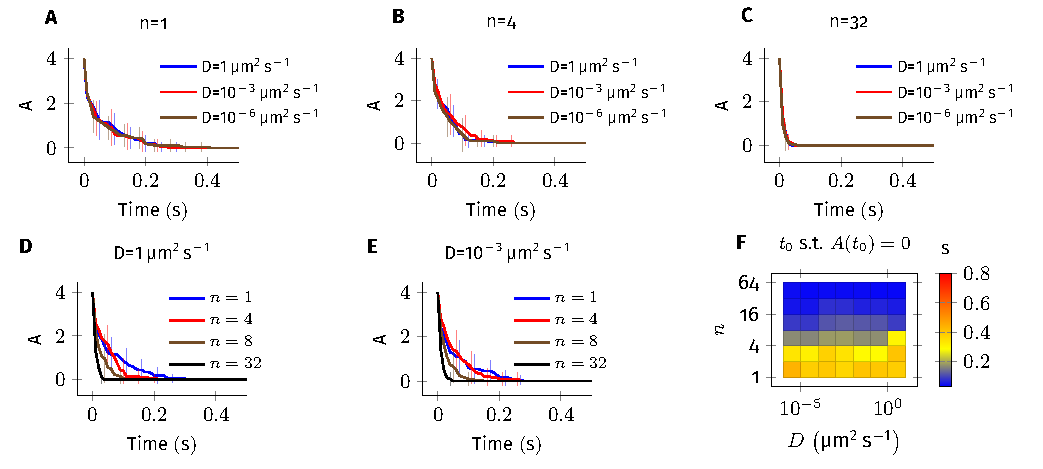
\includegraphics[width=\linewidth]{PaperFigures/suppl/figure_bimolecular_reac_rdme.pdf}\label{si:fig:discretization}
    \captionof{figure}{Error estimate for the bimolecular reaction
        $A+B\xrightarrow{k} \phi$ where
        $k=\SI{1e3}{\meter\cubed\per\mole\per\second}$. The values of parameters
        used in this system are similar to the reaction \EQ{dephosphorylation} in main text. 
        4 molecules of A and B each  were simulated in a cylinderical arena 
        of length $L$=\SI{500}{\nano\meter} and radius $r$=\SI{20}{\nano\meter}. 
        This arena is divided into $n$ equal subvolumes, each of length $h=L/n$. 
        Diffusion of A and B is implemented as described in
        \EQ{discrete} in \nameref{subsec:rdme} where $D_A=D_B=D$.
        {\bf(A,B,C,D,E)} Average of 20 trajectories of A vs time (error bars are
        standard-deviation) for different combinations of $n$ and $D$. For fixed
        value of $n$, kinetics are undistinguishable from each other for non-zero
        value of $D$ (A, B and C). This suggests that the results described in 
        \FIGSUPP[subunit_facilitates_spread]{diffusion_reduces_pp1_potency} are
        not majorly due to computational errors. For fixed value of $D$, however, 
        changing $n$ has huge impact on dynamics of A (D,E) especially when there 
        is less than 1 molecule in each voxel (compare plots where n=1,4 vs n=8,16). 
        {\bf(F)} Time for A to reach zero ($t_0$) vs $D$ and $n$. 
    }\label{fig:suppl_reac_rdme}
\end{center}

\end{appendixbox}

\end{document}
